\chapter{System Analysis}

\section{Overview}
This chapter presents the requirements analysis and modeling artifacts for \projectname. It identifies the system stakeholders, defines the functional and non-functional requirements, and documents the system structure through use case descriptions, an entity-relationship diagram, a class diagram, and process diagrams. These artifacts establish the scope and constraints that guide the design and implementation described in subsequent chapters.

\section{Stakeholders}
The system serves five primary stakeholder groups, each with distinct goals and interaction patterns:

\begin{itemize}[leftmargin=*]
    \item \textbf{Shoppers (End Users).} Consumers who browse products, use virtual try-on and body measurement features, interact with the AI fashion assistant, participate in the community, and complete purchases. They expect personalized recommendations, accurate size guidance, realistic garment visualization, and a seamless bilingual interface.

    \item \textbf{Merchants.} Business owners who register merchant accounts, list products with images and size charts, manage inventory and pricing, fulfill orders, and monitor sales through a merchant dashboard. They require tools for product management, order processing, and customer communication.

    \item \textbf{Customer Service Representatives.} Support agents assigned to branches who handle user inquiries through a ticketing system. They receive, respond to, and resolve support tickets with prioritized workflows (open, assigned, resolved, closed). Each agent has a customer service profile linked to a specific branch, and they communicate with users through threaded ticket messages with unread tracking.

    \item \textbf{Designers.} Users with the designer role who submit original design concepts for community review. Designs go through an approval workflow (pending, approved, in production, published, rejected) managed by administrators. Designers benefit from community feedback through upvotes, downvotes, and comments.

    \item \textbf{System Administrators.} Platform operators who manage user accounts, moderate community content, approve or reject designer submissions, oversee support operations, and monitor system health across all services.
\end{itemize}

\section{Functional Requirements}

The functional requirements are organized by subsystem to reflect the modular architecture.

\subsection{Authentication and User Management}
\begin{enumerate}[leftmargin=*, label=FR-\arabic*.]
    \item The system shall support user registration with email, password, phone, and OTP verification.
    \item The system shall support login via local credentials and Google OAuth.
    \item The system shall issue JWT access tokens and refresh tokens for session management.
    \item The system shall support password reset via email OTP.
    \item The system shall enforce role-based access control with five roles: user, merchant, admin, customer service, and designer.
    \item The system shall allow users to manage their profile, including profile image, body measurements (height, weight), and a dedicated try-on image.
\end{enumerate}

\subsection{Marketplace and E-Commerce}
\begin{enumerate}[leftmargin=*, label=FR-\arabic*., resume]
    \item Merchants shall be able to create, update, and delete product listings with name, description, price, sale price, images, sizes, colors, material, brand, tags, styles, occasions, and size measurement charts.
    \item Products shall support gender categorization (male, female, unisex) and garment type classification.
    \item Shoppers shall be able to browse products with filtering by category, type, brand, price range, color, and size.
    \item Shoppers shall be able to add products to a shopping cart with size and color selection.
    \item The system shall support order creation with delivery address and payment method, order status tracking, and order history.
    \item Shoppers shall be able to submit product reviews with ratings (0.5--5 stars), text comments, likes, and threaded replies.
    \item Shoppers shall be able to add products, posts, and designs to a wishlist with optional notes.
    \item Merchants shall have a dashboard for managing products, viewing orders, and tracking sales.
\end{enumerate}

\subsection{Community and Social Features}
\begin{enumerate}[leftmargin=*, label=FR-\arabic*., resume]
    \item Users shall be able to create community posts of types: issue, review, tip, or question, with title, content, and optional images.
    \item Designers shall be able to submit design proposals with name, description, category, and price.
    \item Users shall be able to comment on posts and designs, with support for threaded replies (parent--child comments).
    \item Users shall be able to vote on posts (like), designs (upvote/downvote), and comments (like).
    \item Users shall be able to follow and unfollow other users, with follower and following counts maintained on user profiles.
    \item The system shall generate notifications for social interactions: likes, comments, replies, votes, design status changes, and new followers.
\end{enumerate}

\subsection{Virtual Try-On}
\begin{enumerate}[leftmargin=*, label=FR-\arabic*., resume]
    \item The system shall accept a person image and a garment image and generate a 2D virtual try-on result using diffusion-based synthesis.
    \item The system shall support multi-angle try-on, generating results from front, right, left, and back viewpoints.
    \item The system shall preprocess person inputs (video or images) through a DensePose and human parsing pipeline to produce conditioning data.
    \item The system shall accept garment front and back images and prepare them for the multiview pipeline.
    \item The system shall support a full multiview try-on workflow: preprocessing, dataset construction, model inference, and result retrieval.
    \item The system shall persist try-on results with metadata (model type, product reference, garment category) and support history retrieval per user.
\end{enumerate}

\subsection{Body Measurement and Size Recommendation}
\begin{enumerate}[leftmargin=*, label=FR-\arabic*., resume]
    \item The system shall estimate body measurements (chest, waist, hip, shoulder, neck, arm length, trouser length, thigh) from a single front-facing photograph.
    \item The system shall accept user-provided height and weight for calibration and apply weight-based circumference correction when the predicted mass deviates significantly.
    \item The system shall map estimated measurements to size recommendations across multiple regional size charts (EU, US, UK, IT, FR, DE) with configurable fit preferences (regular, slim, oversized).
    \item The system shall persist measurement results per user with confidence scores and processing metadata.
\end{enumerate}

\subsection{360-Degree Visualization}
\begin{enumerate}[leftmargin=*, label=FR-\arabic*., resume]
    \item The system shall generate 360-degree interactive previews from multiview try-on outputs using Gaussian splatting reconstruction.
    \item The system shall expose status and health endpoints for the reconstruction service.
\end{enumerate}

\subsection{AI Fashion Assistant (RAG)}
\begin{enumerate}[leftmargin=*, label=FR-\arabic*., resume]
    \item The system shall classify user messages into categories: product search, greeting, follow-up, non-fashion, or clarification.
    \item The system shall extract structured intent attributes (garment type, colors, budget, sizes, brands, occasion, gender) from natural language messages.
    \item The system shall retrieve candidate products using hybrid search: metadata filtering followed by semantic ranking with a configurable similarity threshold.
    \item The system shall assemble retrieved products into complete outfit recommendations.
    \item The system shall generate bilingual (Arabic and English) natural language responses grounded in retrieved catalog data.
    \item The system shall maintain per-user conversation history for multi-turn interactions.
    \item The system shall provide profile-aware styling guidance using a knowledge base that accounts for height, weight, age, and gender.
\end{enumerate}

\section{Non-Functional Requirements}

\begin{longtable}{p{3.5cm} p{10cm}}
\toprule
\textbf{Category} & \textbf{Requirement} \\
\midrule
\endfirsthead
\toprule
\textbf{Category} & \textbf{Requirement} \\
\midrule
\endhead
\bottomrule
\endfoot

Reliability &
The system shall implement health check endpoints for all AI services. Failed service dependencies shall be reported at startup without preventing other services from operating. Global exception handlers shall catch and log unhandled errors with structured error responses. \\

Performance &
Interactive endpoints (product browsing, cart, orders) shall respond within 500ms. AI inference endpoints (try-on, measurements) shall complete within 60 seconds. The RAG pipeline shall respond within 10 seconds for typical queries. The 360 rendering component shall support real-time frame rates. \\

Security &
All sensitive endpoints shall require JWT authentication. Passwords shall be hashed using bcrypt. Rate limiting shall be applied to authentication and API endpoints. CORS shall restrict origins to authorized frontends. Input validation shall be enforced on all endpoints using schema-based validation (Zod). The system shall enforce HTTPS in production and apply security headers. \\

Scalability &
Services shall be independently deployable and horizontally scalable. The backend shall support concurrent connections through connection pooling and async I/O. MongoDB indexes shall be defined for all frequent query patterns. \\

Maintainability &
The codebase shall follow a modular architecture with clear separation between routes, controllers, services, and models. Each backend module shall follow a consistent file structure. Configuration shall be externalized through environment variables. \\

Usability &
The frontend shall support Arabic and English with locale-based routing and RTL layout. The interface shall be responsive across desktop and mobile viewports. The AI assistant shall detect input language and respond in the same language. \\

\end{longtable}

\section{Use Case Model}

This section describes the primary use cases that define user interactions with \projectname. Figure~\ref{fig:usecase} presents the use case diagram.

\begin{figure}[H]
    \centering
    % \includegraphics[width=\textwidth]{figures/use-case-diagram.png}
    \includegraphics[width=0.9\textwidth]{figures/usecase.png}
    \caption{Use case diagram for \projectname.}
    \label{fig:usecase}
\end{figure}

\subsection{UC-1: Browse and Purchase Products}
\begin{tabular}{p{3.5cm} p{10cm}}
\toprule
\textbf{Actor} & Shopper \\
\textbf{Precondition} & User is registered and logged in. \\
\textbf{Main Flow} &
1. User browses the shop with optional filters (category, price, color, size, brand). \newline
2. User selects a product and views details, images, reviews, and size chart. \newline
3. User selects size and color, adds product to cart. \newline
4. User proceeds to checkout, enters delivery address and payment method. \newline
5. System creates the order and decrements product stock. \newline
6. User receives order confirmation. \\
\textbf{Postcondition} & Order is created with status ``pending.'' Stock is updated. \\
\textbf{Alternate Flow} & If product is out of stock, system displays an error and prevents adding to cart. \\
\bottomrule
\end{tabular}

\vspace{1em}

\subsection{UC-2: Virtual Try-On}
\begin{tabular}{p{3.5cm} p{10cm}}
\toprule
\textbf{Actor} & Shopper \\
\textbf{Precondition} & User has uploaded a profile try-on image or provides one during the session. \\
\textbf{Main Flow} &
1. User navigates to the virtual try-on page. \newline
2. User selects or uploads a person image and a garment image. \newline
3. System sends images to the try-on service. \newline
4. Try-on service preprocesses inputs and runs diffusion-based synthesis. \newline
5. System returns the generated try-on result image. \newline
6. Result is saved to the user's try-on history. \\
\textbf{Postcondition} & Try-on result is displayed and persisted in history. \\
\textbf{Alternate Flow} & If the try-on service is unavailable, system displays a service status message. \\
\bottomrule
\end{tabular}

\vspace{1em}

\subsection{UC-3: Body Measurement and Size Recommendation}
\begin{tabular}{p{3.5cm} p{10cm}}
\toprule
\textbf{Actor} & Shopper \\
\textbf{Precondition} & User has a front-facing full-body photograph. \\
\textbf{Main Flow} &
1. User uploads a front-facing photograph. \newline
2. User enters their height (required) and weight (optional). \newline
3. User selects gender, region (EU/US/UK), and fit preference. \newline
4. System sends the image and parameters to the SHAPY measurement service. \newline
5. Service estimates body measurements from the 3D mesh regression output. \newline
6. System maps measurements to size recommendations and returns results with confidence scores. \\
\textbf{Postcondition} & Measurements and size recommendation are displayed and saved to user profile. \\
\textbf{Alternate Flow} & If SHAPY service is unavailable, system informs the user and suggests retrying later. \\
\bottomrule
\end{tabular}

\vspace{1em}

\subsection{UC-4: AI Fashion Assistant Chat}
\begin{tabular}{p{3.5cm} p{10cm}}
\toprule
\textbf{Actor} & Shopper \\
\textbf{Precondition} & None (assistant is accessible without login for basic queries). \\
\textbf{Main Flow} &
1. User opens the fashion assistant chat interface. \newline
2. User sends a natural language message (Arabic or English). \newline
3. System classifies the message intent. \newline
4. For product searches: system extracts structured attributes, retrieves matching products via hybrid search, assembles outfit recommendations, and generates a natural language response. \newline
5. Response is displayed with product cards and explanations. \\
\textbf{Postcondition} & Conversation turn is persisted for multi-turn context. \\
\textbf{Alternate Flow} & For greetings, non-fashion, or ambiguous queries, the system responds with appropriate fixed messages or clarification questions. \\
\bottomrule
\end{tabular}

\vspace{1em}

\subsection{UC-5: Community Participation}
\begin{tabular}{p{3.5cm} p{10cm}}
\toprule
\textbf{Actor} & Shopper, Designer \\
\textbf{Precondition} & User is registered and logged in. \\
\textbf{Main Flow} &
1. User creates a post (issue, review, tip, or question) with title, content, and optional images. \newline
2. Other users view, like, and comment on the post. \newline
3. Post author and commenters receive notifications for interactions. \newline
4. Users can follow other users to stay updated on their activity. \\
\textbf{Postcondition} & Post is published, engagement counters are updated, and notifications are dispatched. \\
\textbf{Alternate Flow} & Designer-specific flow: designer submits a design proposal, which enters the admin approval pipeline before becoming visible to the community. \\
\bottomrule
\end{tabular}

\vspace{1em}

\subsection{UC-6: Merchant Product Management}
\begin{tabular}{p{3.5cm} p{10cm}}
\toprule
\textbf{Actor} & Merchant \\
\textbf{Precondition} & User has the merchant role and a registered merchant profile. \\
\textbf{Main Flow} &
1. Merchant accesses the merchant dashboard. \newline
2. Merchant creates a new product listing with all required attributes (name, description, price, images, sizes, colors, material, brand). \newline
3. Merchant optionally adds a size measurement chart mapping sizes to body measurements. \newline
4. Merchant manages existing listings: updates stock, adjusts prices, adds sale prices, or deactivates products. \newline
5. Merchant views and processes incoming orders. \\
\textbf{Postcondition} & Product listings are updated and immediately reflected in the storefront and search results. \\
\bottomrule
\end{tabular}

\section{Data Model and Entity-Relationship Diagram}

The system uses MongoDB as its primary data store. While MongoDB is a document-oriented database without enforced relational schemas, the application layer defines structured document schemas using Mongoose. The following entity-relationship diagram illustrates the logical relationships between the core entities.

\begin{figure}[H]
    \centering
    % 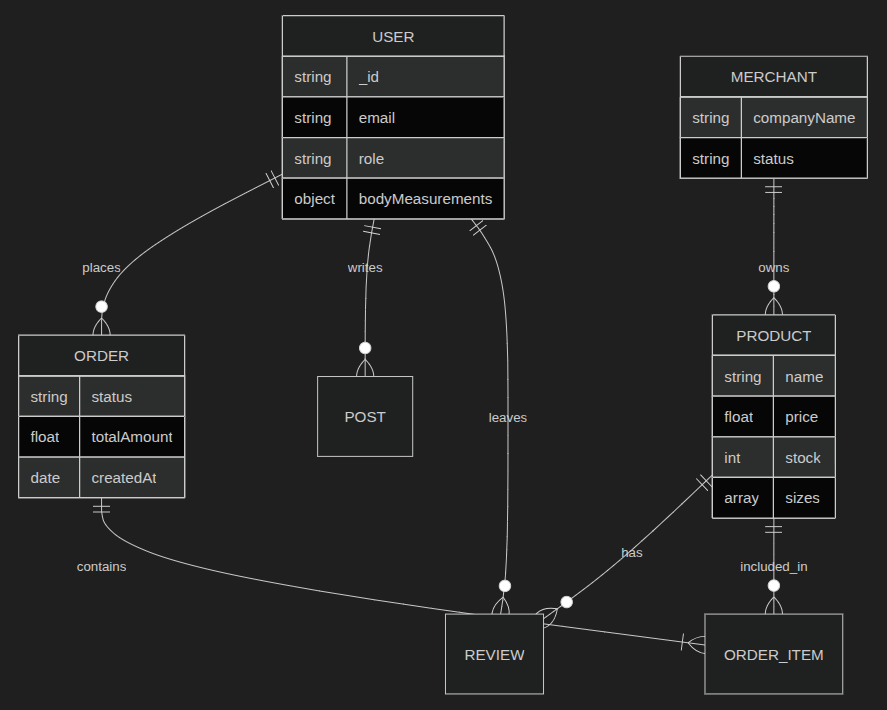
\includegraphics[width=\textwidth]{figures/erd.png}
    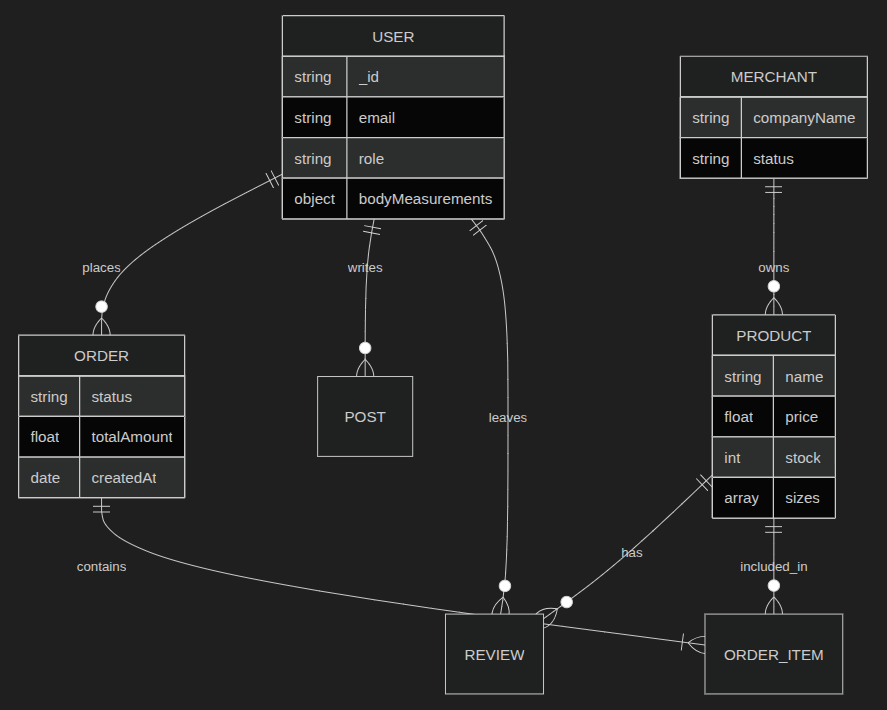
\includegraphics[width=\textwidth]{figures/erd.png}
    \caption{Entity-relationship diagram for \projectname.}
    \label{fig:erd}
\end{figure}

\subsection{Core Entities}

\textbf{User.} The central entity representing all platform users. Key attributes include name, email (with normalized duplicate), password (hashed, select-excluded), phone, address, birth date, role (user/merchant/admin/cs/designer), authentication provider (local/Google), profile images, body measurement fields (height\_cm, weight\_kg), a dedicated try-on image, account status flags (isActive, isSuspended), social counters (followersCount, followingCount), session tracking, and token management fields (tokenVersion, refreshToken, resetOTP).

\textbf{Product.} Represents a marketplace listing. Key attributes include name, description, price, sale price, stock count, merchant reference, category, garment type, image URLs, tags, available sizes, a size measurement chart (array of size-to-measurement mappings for chest, waist, hip, shoulder, inseam), colors, gender, material, brand, styles, occasions, and view count. Products are indexed on category, type, brand, price, merchant, tags, colors, and a text index on name, description, and brand for full-text search.

\textbf{Order.} Captures a purchase transaction. Contains a user reference, an array of order items (each with product reference, quantity, price, selected size, and selected color), total amount, status, delivery address, and payment method.

\textbf{MerchantProfile.} Extends a user with merchant-specific data: company name, company ID, national ID, and a list of product references.

\textbf{Review.} A product review containing user reference, product reference, rating (0.5--5), comment text, likes (array of user references), and threaded replies.

\textbf{TryOnResult.} Records a virtual try-on session. Contains user and product references, model type (vton2d/prova-vton/multiangle), result image URL and public ID, video generation status and metadata, garment category, and timestamps.

\textbf{BodyMeasurements.} Stores measurement estimation results. Contains user reference, engine used (shapy), source image URLs, input metadata (height, weight, gender, region, fit), the full measurements object, size recommendation, confidence scores, debug information, and processing time.

\subsection{Community Entities}

\textbf{Post.} A community post with author reference, type (issue/review/tip/question), title, content, optional images, optional store reference, optional rating, engagement counters (likesCount, commentsCount), and active status.

\textbf{Design.} A designer submission with name, description, category, price, designer reference, approval status (pending/approved/in\_production/published/rejected), vote counters, admin notes, and a computed virtual field for net votes.

\textbf{Comment.} A polymorphic comment that targets either a post or a design (via targetType and targetId). Supports threaded replies through a parentId self-reference. Tracks likesCount and repliesCount.

\textbf{Vote.} A polymorphic vote entity targeting posts, designs, or comments. Each vote has a type (like/upvote/downvote) and is uniquely constrained per user per target.

\textbf{Follow.} Represents a follower--following relationship between two users with a unique constraint preventing duplicate follows and a pre-save hook preventing self-follows.

\textbf{Notification.} Event-driven notifications with recipient, sender, type (like\_post, comment\_post, upvote\_design, follow, etc.), target reference, message text, read status, and a 30-day TTL auto-expiry index.

\textbf{Wishlist.} A polymorphic bookmark entity allowing users to save products, posts, or designs with optional notes. Uniquely constrained per user per item type and ID.

\textbf{SupportTicket.} Represents a customer service interaction. Contains user reference and contact details, optional agent assignment, status (open/assigned/resolved/closed), subject, priority (low/medium/high), a threaded messages array (each message with sender ID, name, role, content, and timestamp), last message preview, and unread counters for both user and agent sides.

\textbf{CustomerServiceProfile.} Extends a user with the customer service role. Links the agent to a specific branch for organizational routing.

\subsection{Key Relationships}
\begin{itemize}[leftmargin=*]
    \item A \textbf{User} has zero or more \textbf{Orders}, \textbf{Reviews}, \textbf{TryOnResults}, \textbf{BodyMeasurements}, \textbf{Posts}, \textbf{Designs}, \textbf{Comments}, \textbf{Votes}, \textbf{Wishlists}, and \textbf{Notifications}.
    \item A \textbf{Merchant} (User with merchant role) has one \textbf{MerchantProfile} and zero or more \textbf{Products}.
    \item A \textbf{Product} belongs to one \textbf{Merchant} and has zero or more \textbf{Reviews} and \textbf{OrderItems}.
    \item An \textbf{Order} belongs to one \textbf{User} and contains one or more \textbf{OrderItems}, each referencing a \textbf{Product}.
    \item A \textbf{Comment} belongs to one \textbf{User} and targets one \textbf{Post} or \textbf{Design}. Comments may have a parent \textbf{Comment} for threading.
    \item A \textbf{Vote} belongs to one \textbf{User} and targets one \textbf{Post}, \textbf{Design}, or \textbf{Comment}.
    \item A \textbf{Follow} connects two \textbf{Users} (follower and following).
\end{itemize}

\section{Class Diagram}

The class diagram illustrates the major software components and their relationships across the backend and AI services.

\begin{figure}[H]
    \centering
    % \includegraphics[width=\textwidth]{figures/class-diagram.png}
    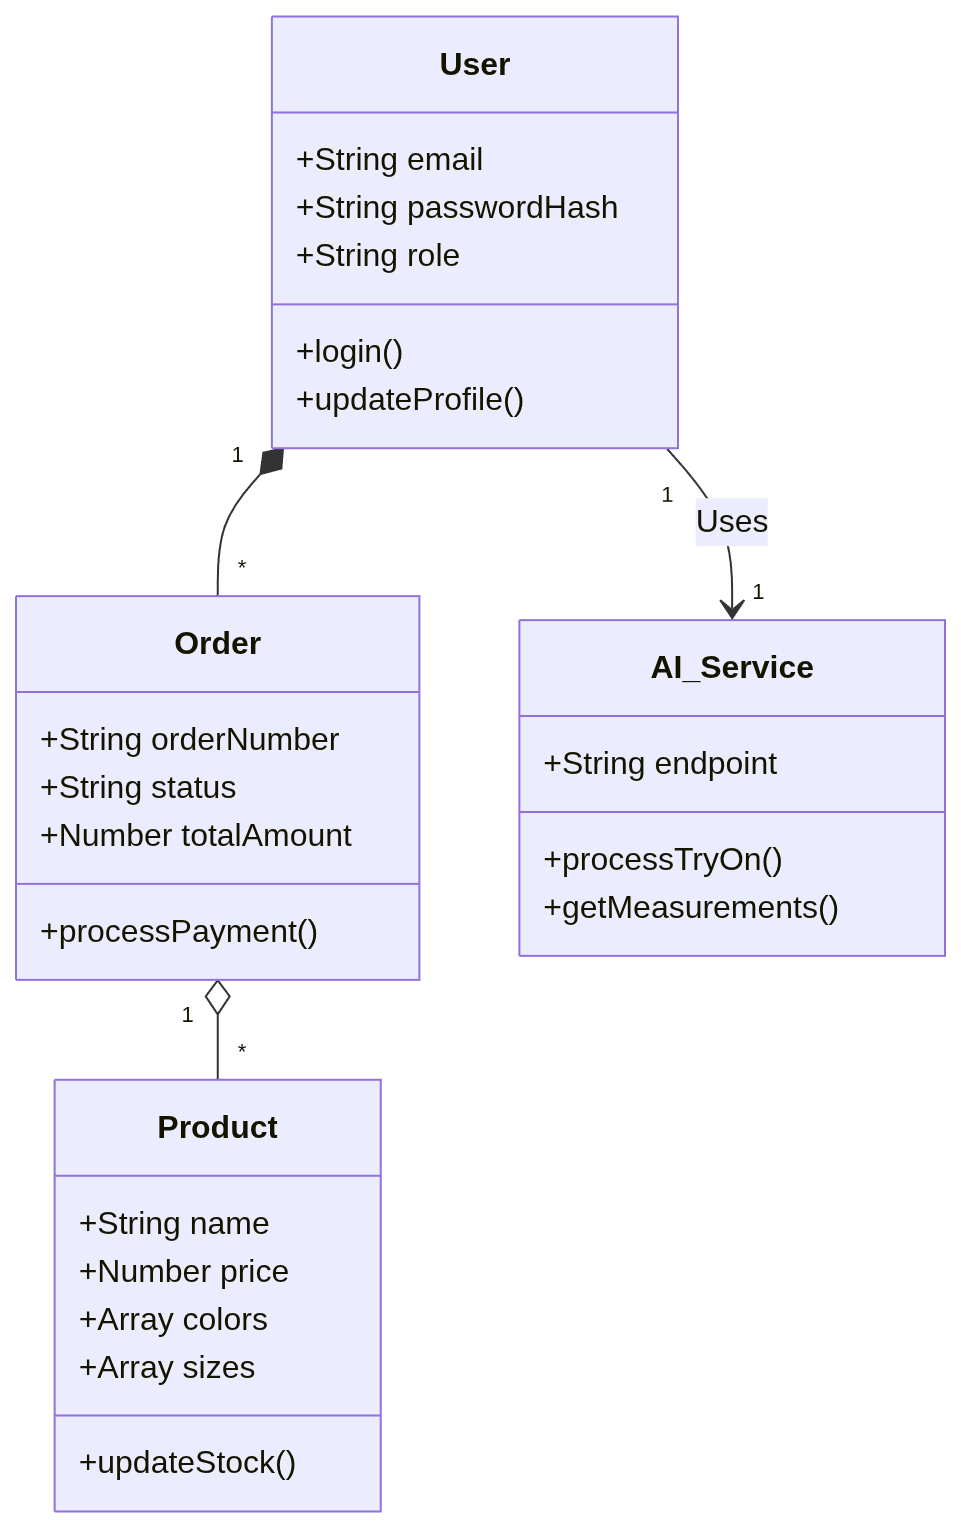
\includegraphics[width=\textwidth]{figures/classdiagram.png}
    \caption{Class diagram showing major components of \projectname.}
    \label{fig:classdiagram}
\end{figure}

The backend follows a layered module pattern. Each domain module (auth, product, order, post, etc.) contains four components: a \textbf{Routes} file that defines HTTP endpoints and attaches middleware, a \textbf{Controller} that handles request parsing and response formatting, a \textbf{Service} that implements business logic, and a \textbf{Model} that defines the Mongoose schema and database interface. Validation is handled by \textbf{Schema} files using Zod. Cross-cutting concerns—authentication, rate limiting, CORS, security headers, logging, and error handling—are implemented as Express middleware.

The try-on service follows a similar layered pattern using FastAPI. \textbf{Routers} define API endpoints, \textbf{Services} (ColabClient, MultiAngleClient, MultiviewClient, SHAPYClient, VideoPreprocessor) implement the AI pipeline logic, and \textbf{Models} define request/response schemas using Pydantic. A \textbf{Dependencies} module provides dependency injection for service instances, and a centralized \textbf{ClientState} singleton manages the lifecycle of all external service clients.

The RAG service is organized as a pipeline of composable stages: MessageClassifier, IntentExtractor, ProductRetriever, OutfitAssembler, and ResponseComposer, coordinated by a Pipeline orchestrator. Configuration, embeddings, prompts, and schemas are separated into dedicated modules.

\section{Process and Sequence Diagrams}

This section documents the key processes in the system using sequence diagrams that trace the flow of data and control across service boundaries.

\subsection{Product Purchase Flow}
\begin{figure}[H]
    \centering
    % 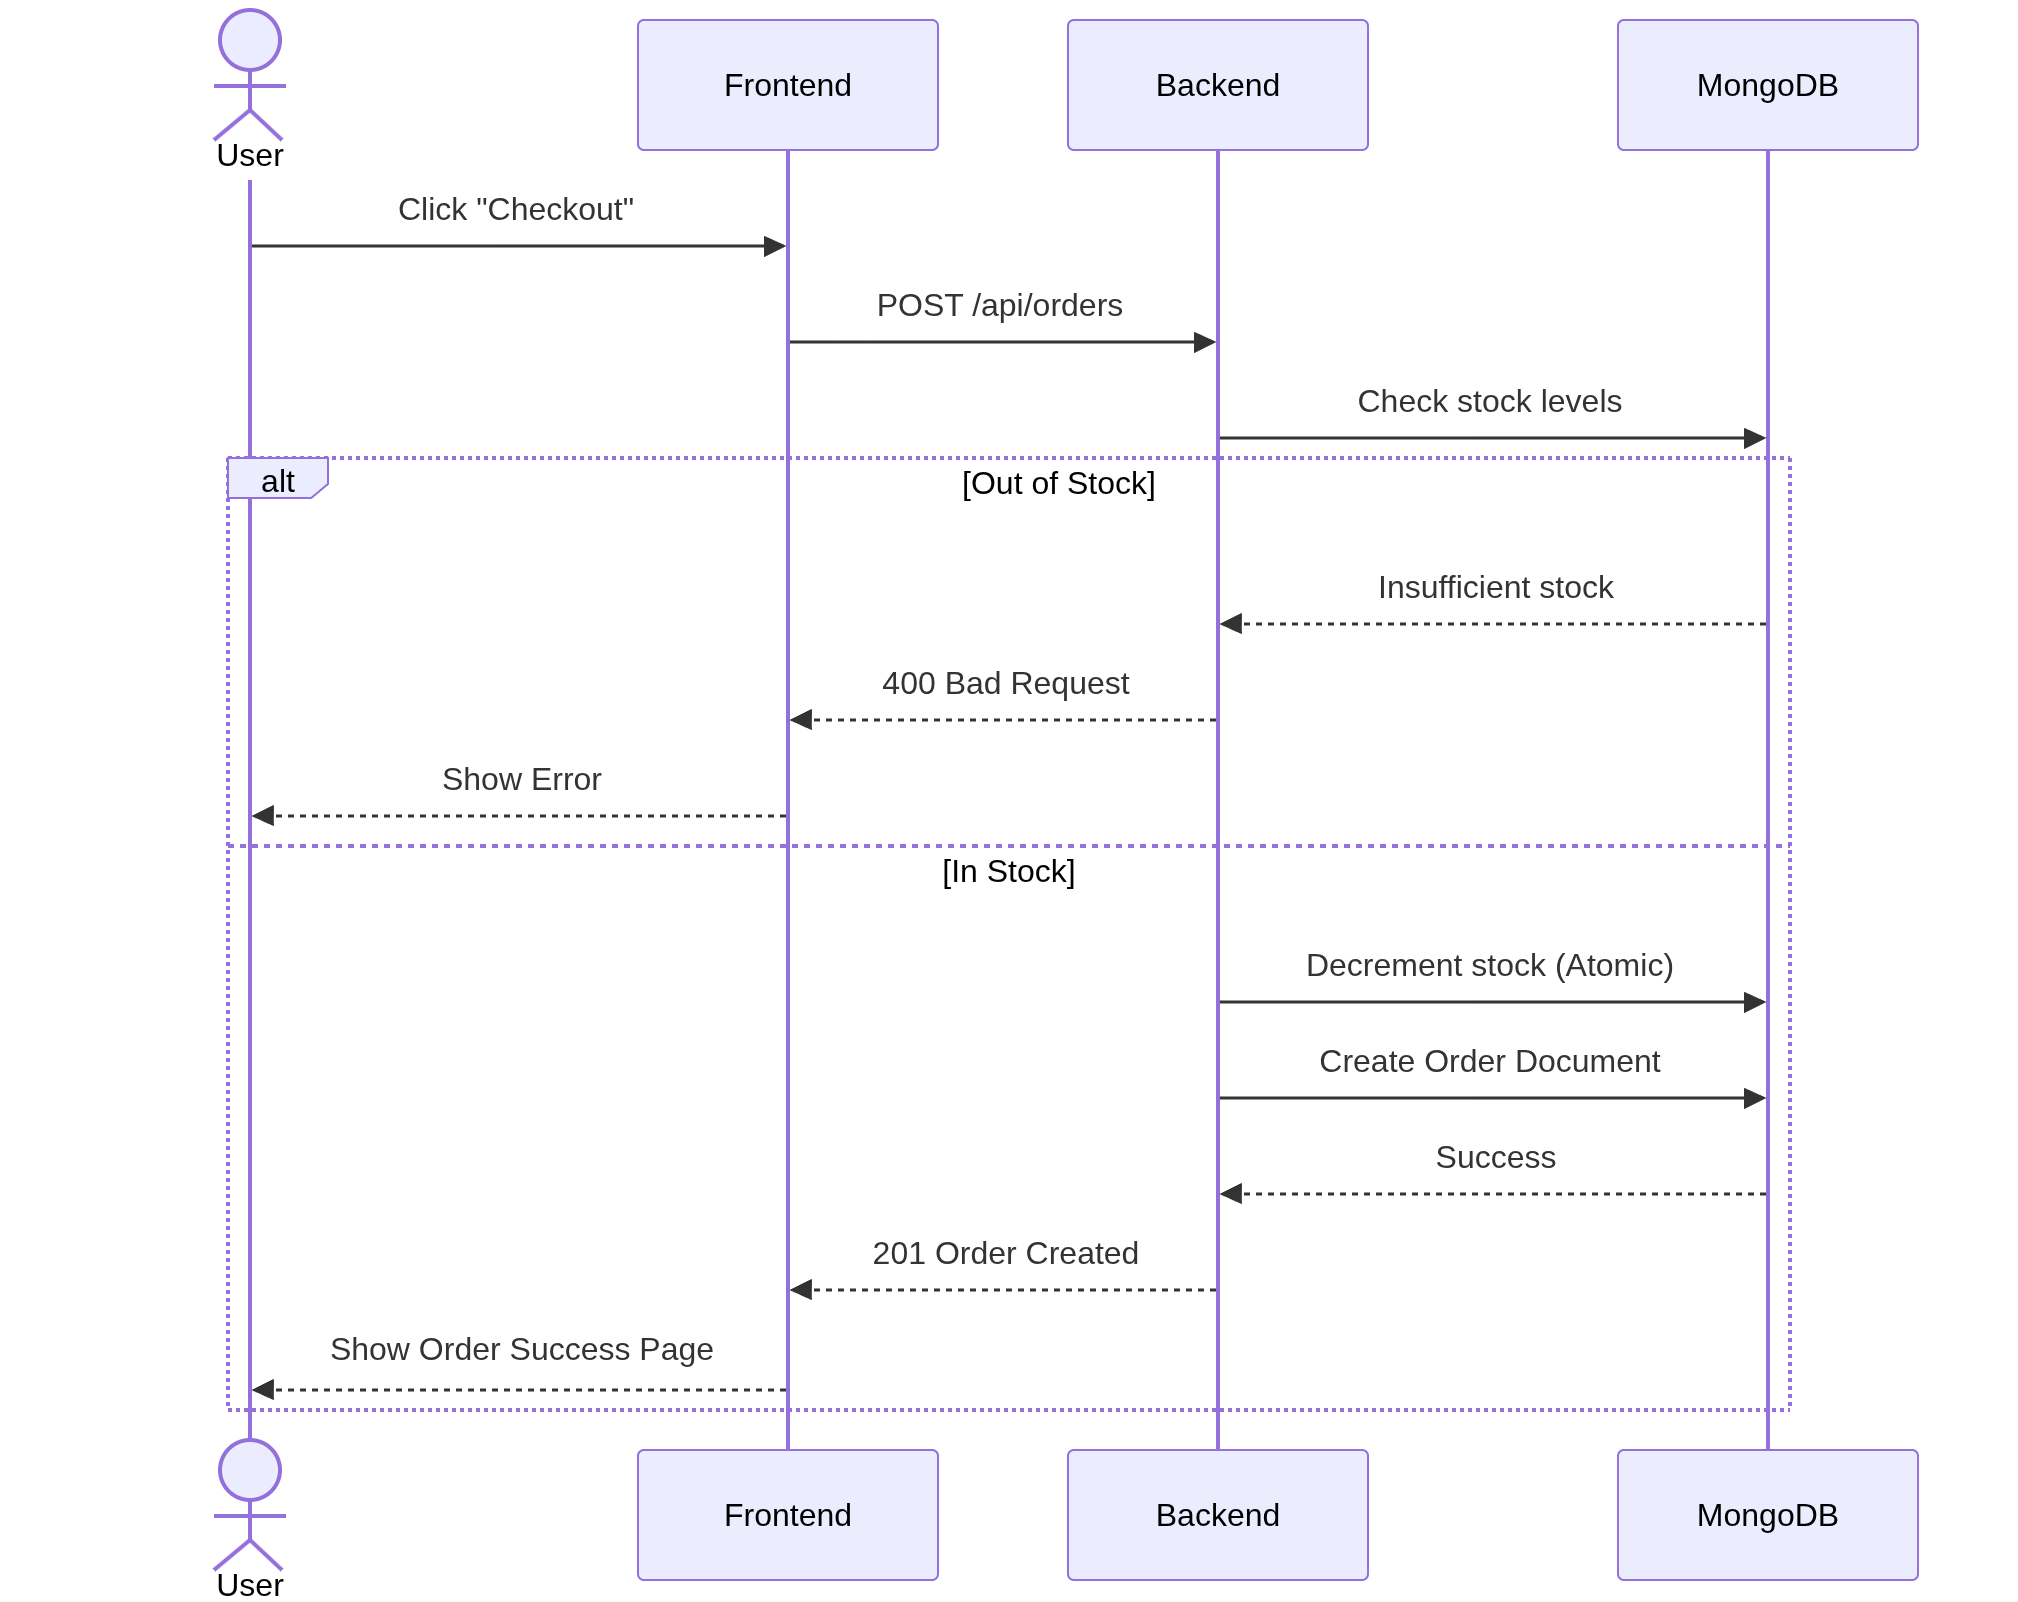
\includegraphics[width=\textwidth]{figures/seq-purchase.png}
    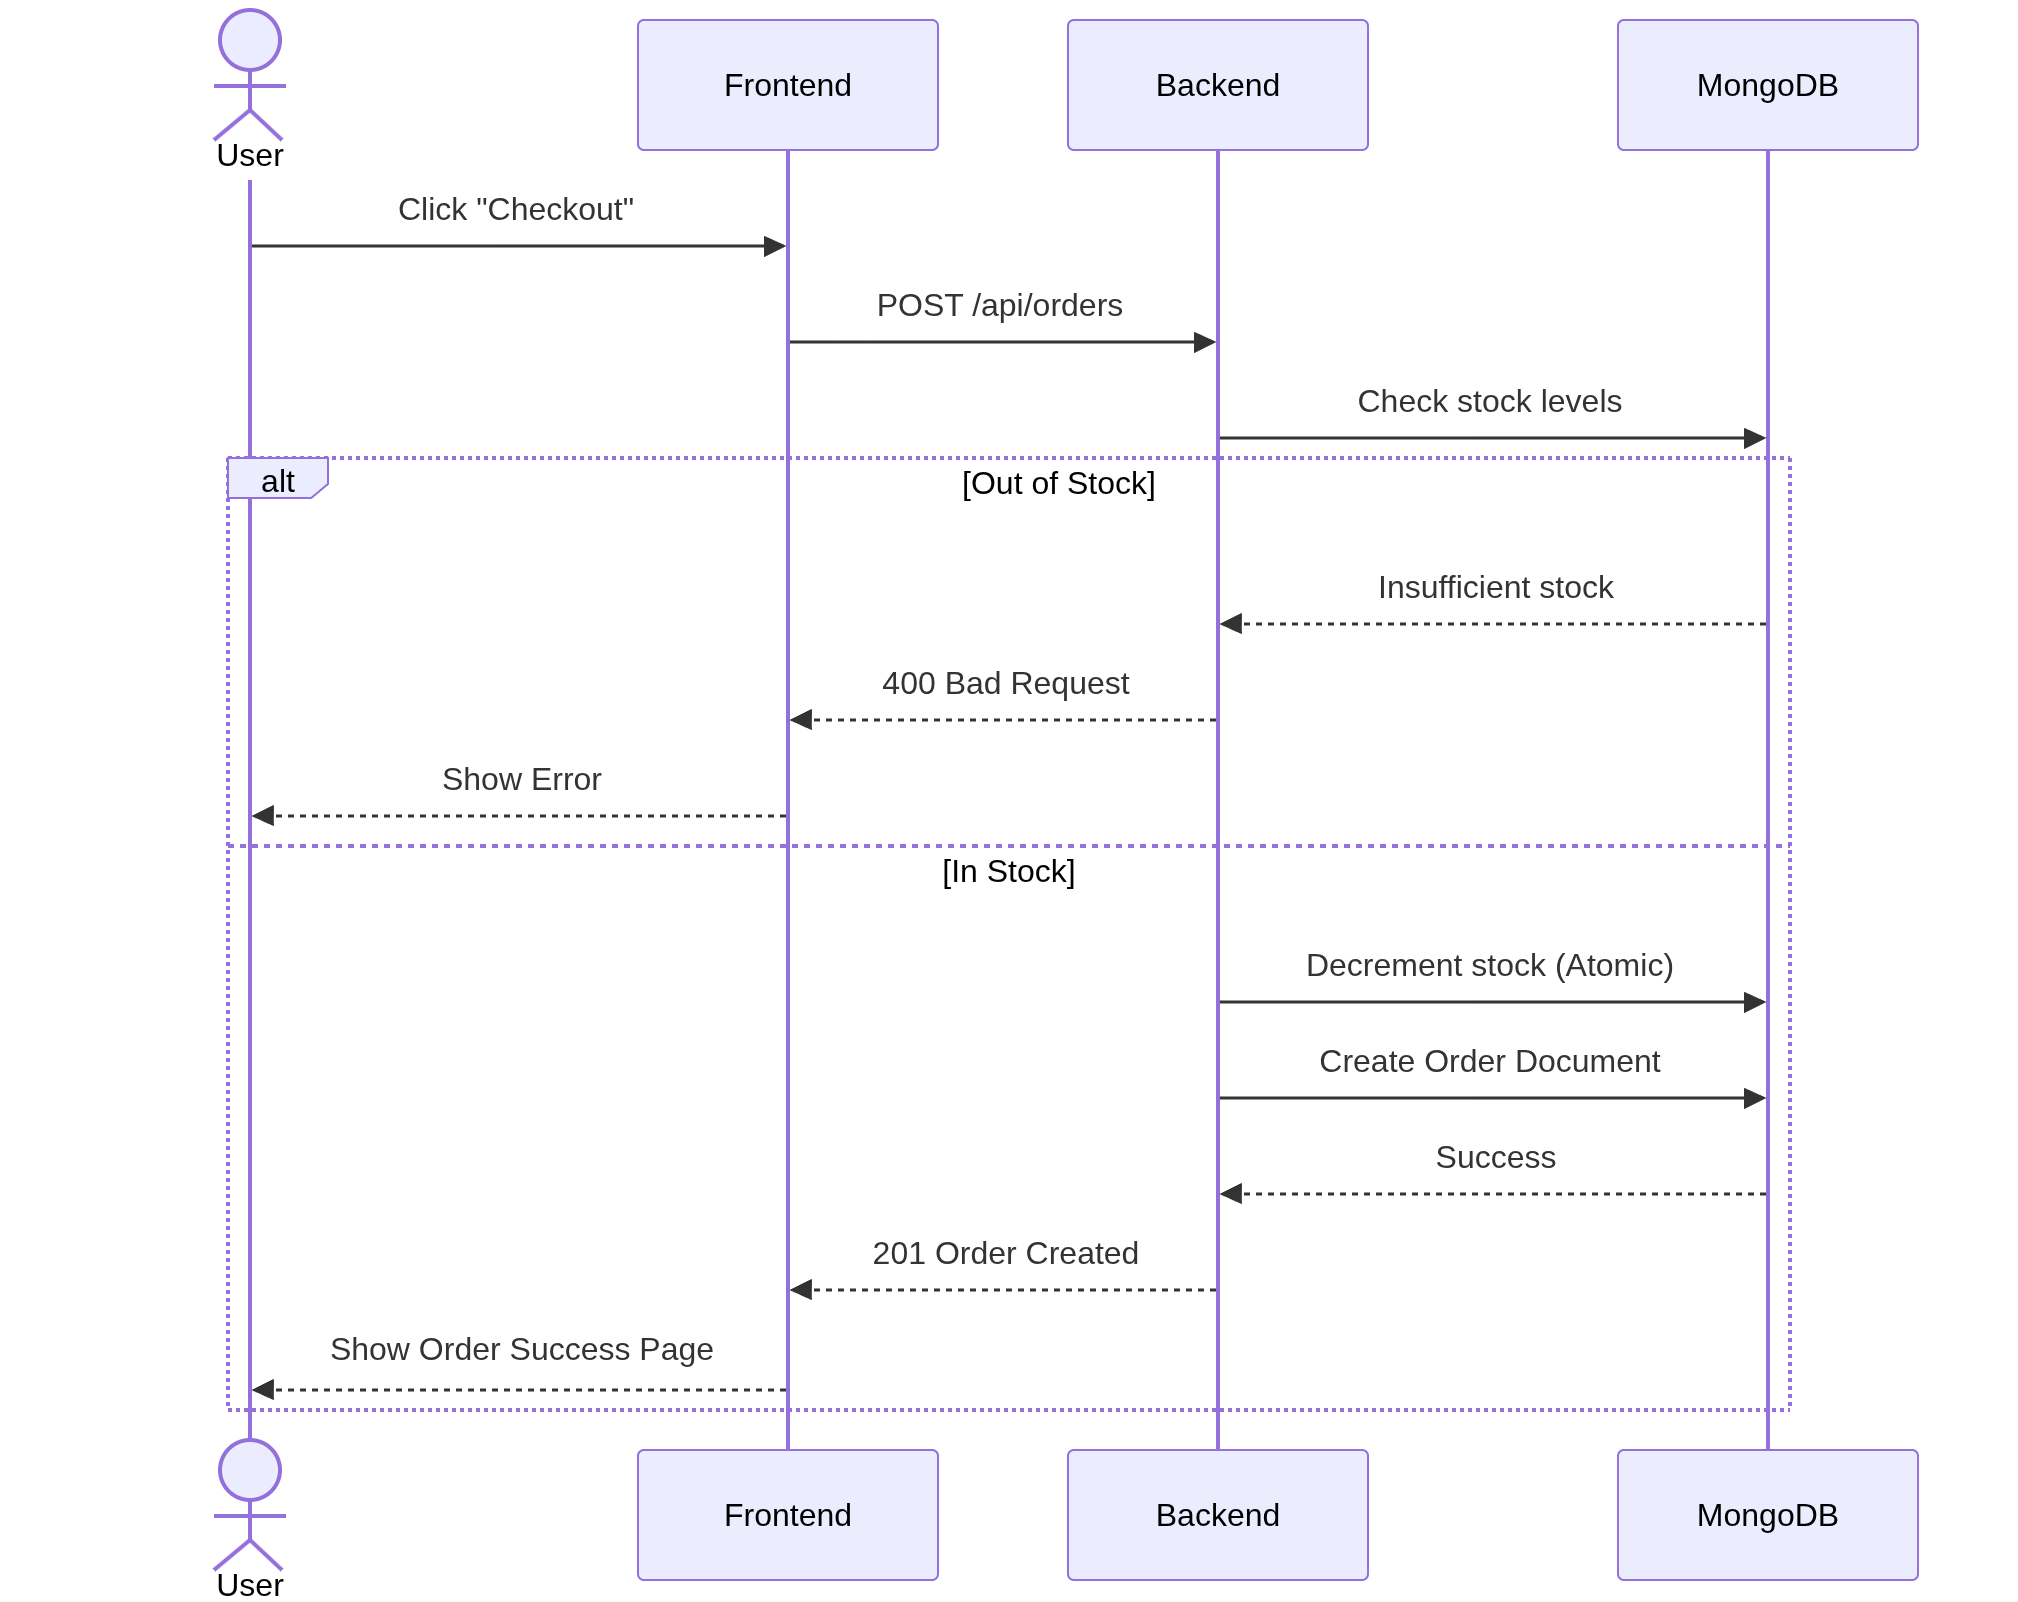
\includegraphics[width=0.9\textwidth]{figures/seq-purchase.png}
    \caption{Sequence diagram for the product purchase flow.}
    \label{fig:seq-purchase}
\end{figure}

The purchase flow proceeds as follows: (1) the shopper adds items to their cart on the frontend, (2) at checkout, the frontend sends a POST request to the backend order endpoint with items, address, and payment method, (3) the backend validates stock availability for each item, (4) the backend creates the order document and decrements stock for each product atomically, (5) the backend returns the order confirmation to the frontend, and (6) the frontend navigates to the order success page. If any item is out of stock, the backend returns a validation error before creating the order.

\subsection{Virtual Try-On Flow}
\begin{figure}[H]
    \centering
    % \includegraphics[width=\textwidth]{figures/seq-tryon.png}
    \includegraphics[width=0.9\textwidth]{figures/seq-tryon.png}
    \caption{Sequence diagram for the 2D virtual try-on flow.}
    \label{fig:seq-tryon}
\end{figure}

The 2D try-on flow involves three services: (1) the frontend uploads person and garment images to the backend, (2) the backend proxies the request to the try-on FastAPI service, (3) the try-on service validates and preprocesses both images, (4) the service sends the images to the custom trained diffusion model (Prova-VTON) for synthesis, (5) the result image is returned to the backend, (6) the backend uploads the result to cloud storage (Cloudinary), saves a TryOnResult document, and returns the image URL to the frontend.

\subsection{RAG Fashion Assistant Flow}
\begin{figure}[H]
    \centering
    % \includegraphics[width=\textwidth]{figures/seq-rag.png}
    \includegraphics[width=0.9\textwidth]{figures/seq-rag.png}
    \caption{Sequence diagram for the RAG fashion assistant pipeline.}
    \label{fig:seq-rag}
\end{figure}

The RAG flow proceeds through five stages: (1) the frontend sends the user's natural language message to the chat service, (2) the pipeline classifies the message intent—greetings and non-fashion queries receive immediate responses without retrieval, (3) for product searches, the intent extractor produces a structured query with attributes such as garment type, colors, and budget, (4) the retriever applies metadata filters against MongoDB and then ranks candidates by semantic similarity using Sentence-BERT embeddings, (5) the outfit assembler groups retrieved products into complete outfits, and (6) the response composer generates a bilingual explanation grounded in the actual retrieved products. The conversation turn is appended to the per-user history store for multi-turn context.

\subsection{Body Measurement Flow}
\begin{figure}[H]
    \centering
    % \includegraphics[width=\textwidth]{figures/seq-measurement.png}
    \includegraphics[width=0.9\textwidth]{figures/seq-measurement.png}
    \caption{Sequence diagram for body measurement and size recommendation.}
    \label{fig:seq-measurement}
\end{figure}

The measurement flow involves the following steps: (1) the frontend uploads a front-facing photograph along with height, weight, gender, and region parameters, (2) the backend forwards the request to the try-on service measurement endpoint, (3) the measurement router validates inputs and sends the image to the SHAPY service, (4) SHAPY performs 3D body mesh regression and returns raw shape parameters and circumference estimates, (5) the router applies weight-based circumference correction if the predicted mass deviates significantly from the user-provided weight, (6) derived measurements (widths, lengths) are computed using ISO 7250 anthropometric ratios, (7) the size recommendation module maps chest and waist circumferences to regional size charts with the selected fit preference, and (8) the complete result is returned with confidence scores and persisted to the database.

\subsection{Multiview Try-On and 360 Reconstruction Flow}

The multiview pipeline is the most complex workflow in the system and involves multiple stages across services: (1) the user uploads a video or set of images showing themselves from multiple angles, (2) the preprocessing service extracts frames (if video), runs person detection (YOLOv8), generates DensePose maps, and produces human parsing masks for each frame, (3) the user uploads garment front and back images, which are saved and organized, (4) the system builds a structured dataset ZIP containing the preprocessed person data and cloth images, (5) the ZIP is uploaded to the inference server, (6) the multiview try-on model generates view-consistent results across all viewpoints, (7) results are downloaded and extracted locally, and (8) the multiview outputs can be fed into the Splatfacto Gaussian splatting pipeline to produce an interactive 360-degree reconstruction.

\section{Summary}
This chapter has defined the functional and non-functional requirements for \projectname, identified the stakeholders and their interactions through use cases, documented the data model through entity descriptions and relationships, outlined the software architecture through a class diagram, and traced the key system processes through sequence diagrams. These analysis artifacts establish the foundation for the system design presented in Chapter~4 and the implementation details described in Chapter~5.
